\documentclass[tikz]{standalone}

\usetikzlibrary{positioning, backgrounds}
\usepackage{lmodern}
\usepackage[tracking=true]{microtype}

\newcommand{\tile}[2]{
    \begin{tikzpicture}
% [background rectangle/.style={fill=olive!15}, show background rectangle, inner sep=0pt]    
    \node [shape=rectangle, fill=red, minimum width=2.5cm, minimum height = 3cm] at (current page.north west) (names) {};
    \node[minimum width=2.5cm,minimum height=2.5cm,draw,ultra thick,inner sep = 0pt] at (0,1) {
    \fontsize{60}{60}\selectfont \textbf{\textcolor{#2}{#1}}
    };
    \node[circle,line width=2pt,fill=olive!20,draw=olive!22,minimum size = 30] at (0,-.8){};  
    \end{tikzpicture}
}

\begin{document}
\sffamily

% \tile{2}{red!80}

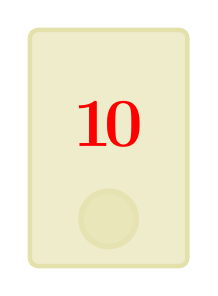
\begin{tikzpicture}
\filldraw [rounded corners=3pt, fill=olive!15, draw=olive!25, ultra thick] (0,0) rectangle (2,3);
\node at (1,1.8) {
    \fontsize{54}{60}\selectfont \textbf{\textcolor{red}{\textls[-100]{10}}}
    };
\node[circle,line width=2pt,fill=olive!20,draw=olive!23,minimum size = 20] at (1,.6){};
\end{tikzpicture}



\end{document}
